\documentclass[tikz,convert={outfile=fonctions.png}]{standalone}

    \usepackage[utf8]{inputenc}

\begin{document}
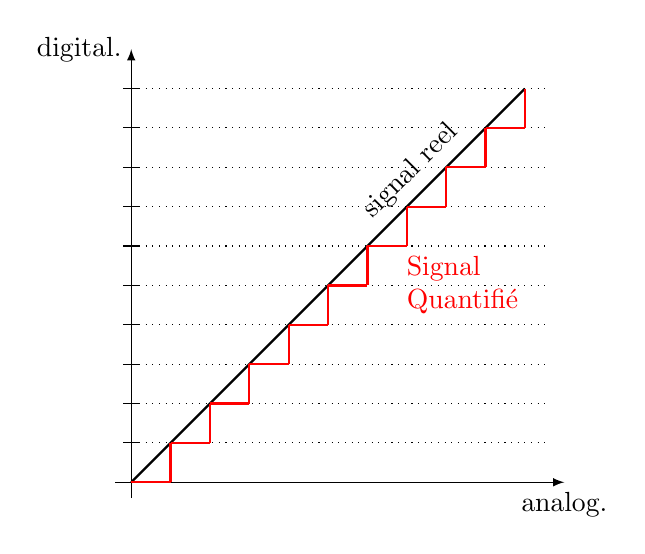
\begin{tikzpicture}[>=latex]

    \draw[->] (-.2,0) -- (5.5,0) node[below] {analog.};
    \draw[->] (0,-.2) -- (0,5.5) node[left] {digital.};

    \foreach \i in{1,...,10} {
        \draw (-.1,\i*.5) -- ++(.2,0);
        \draw[dotted] (.1,\i*.5) -- ++(5.2,0);
    }

    % signal reel
    \draw[thick] (0,0) -- (5,5) node[near end, above, sloped] {signal reel};

    % signal quantifié
    \foreach \i in {0,...,9} {
        \draw[red,thick] (\i*.5,\i*.5) -- ++(.5,0);
        \draw[red,thick] (\i*.5+.5,\i*.5) -- ++(0,.5);

    }
    \draw[red] (4.5,2.5) node[text width=2cm] {Signal Quantifié};

\end{tikzpicture}
\end{document}

